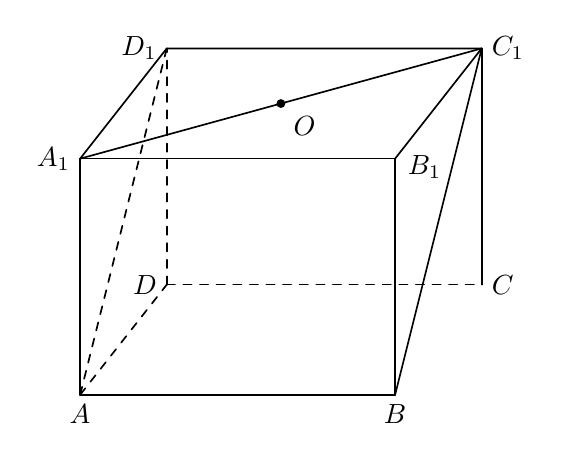
\begin{tikzpicture}[line width=.6pt,line join=round,line cap=round]
% cube projection: front ABB1A1, top A1B1C1D1, bottom ABCD
\coordinate (A) at (0,0);
\coordinate (B) at (4,0);
\coordinate (B1) at (4,3);
\coordinate (A1) at (0,3);
\coordinate (D1) at (1.1,4.4);
\coordinate (C1) at (5.1,4.4);
\coordinate (D) at (1.1,1.4);
\coordinate (C) at (5.1,1.4);
% bottom back (hidden)
\draw[dashed] (D) -- (C);
\draw[dashed] (A) -- (D);
\draw[dashed] (D) -- (D1);
% front face
\draw (A) -- (B) -- (B1) -- (A1) -- cycle;
% top face
\draw (A1) -- (D1) -- (C1) -- (B1);
% right face
\draw (B1) -- (B);
\draw (C) -- (C1);
% plane ABC1D1 edges: A-B already, B-C1, C1-D1 already, D1-A
\draw (B) -- (C1);
\draw[dashed] (A) -- (D1);
% top diagonal with centre O
\draw (A1) -- (C1);
\fill (2.55,3.7) circle (1.6pt);
\node[below right=1pt] at (2.55,3.7) {$O$};
% labels, offset from strokes
\node[below] at (A) {$A$};
\node[below] at (B) {$B$};
\node[right] at (C) {$C$};
\node[left] at (D) {$D$};
\node[left] at (A1) {$A_{1}$};
\node[right,xshift=1pt,yshift=-3pt] at (B1) {$B_{1}$};
\node[right] at (C1) {$C_{1}$};
\node[left] at (D1) {$D_{1}$};
\end{tikzpicture}
